% =====================================================================
%  Jac code-generation fine-tuning -- research review
%  Custom minimal Beamer theme (no external theme dependency).
%  Build:  pdflatex slides.tex   (run TWICE for the table of contents)
% =====================================================================
\documentclass[aspectratio=169,11pt]{beamer}

\usepackage[T1]{fontenc}
\usepackage[utf8]{inputenc}
\usepackage{lmodern}
\usepackage{booktabs}
\usepackage{graphicx}
\usepackage{array}
\usepackage{xcolor}

\usefonttheme{professionalfonts}
\usetheme{default}
\setbeamertemplate{navigation symbols}{}

% ---------------------------------------------------------------- palette
\definecolor{jsPrimary}{HTML}{2F5D75}   % deep petrol -- headings, chrome
\definecolor{jsAccent}{HTML}{2F8F6F}    % teal green  -- "significant" / wins
\definecolor{jsWarm}{HTML}{B5793A}      % ochre       -- caveats / nulls
\definecolor{jsInk}{HTML}{1F2933}       % body text
\definecolor{jsMute}{HTML}{616E7C}      % secondary text
\definecolor{jsRule}{HTML}{C9D2D9}
\definecolor{jsPaper}{HTML}{FCFCFB}

\setbeamercolor{normal text}{fg=jsInk,bg=jsPaper}
\setbeamercolor{structure}{fg=jsPrimary}
\setbeamercolor{frametitle}{fg=jsPrimary,bg=jsPaper}
\setbeamercolor{title}{fg=jsPrimary}
\setbeamercolor{author}{fg=jsMute}
\setbeamercolor{date}{fg=jsMute}
\setbeamercolor{institute}{fg=jsMute}
\setbeamercolor{itemize item}{fg=jsPrimary}
\setbeamercolor{itemize subitem}{fg=jsMute}
\setbeamercolor{alerted text}{fg=jsWarm}
\setbeamercolor{block title}{fg=white,bg=jsPrimary}
\setbeamercolor{block body}{fg=jsInk,bg=jsPrimary!6}
\setbeamercolor{caption name}{fg=jsMute}

\setbeamerfont{frametitle}{size=\large,series=\bfseries}
\setbeamerfont{title}{size=\LARGE,series=\bfseries}
\setbeamerfont{caption}{size=\scriptsize}
\setbeamertemplate{itemize item}{\raisebox{0.12ex}{\scriptsize$\blacksquare$}}
\setbeamertemplate{itemize subitem}{\raisebox{0.15ex}{\tiny$\bullet$}}
\setbeamertemplate{caption}{\insertcaption}

% ------------------------------------------------------- frametitle rule
\makeatletter
\setbeamertemplate{frametitle}{%
  \vspace{0.9em}%
  \begin{beamercolorbox}[wd=\paperwidth,leftskip=0.9cm,rightskip=0.9cm]{frametitle}%
    \usebeamerfont{frametitle}\insertframetitle\par
    \ifx\insertframesubtitle\@empty\else
      {\usebeamerfont*{framesubtitle}\small\color{jsMute}\insertframesubtitle\par}%
    \fi
    \vspace{0.25em}{\color{jsRule}\rule{\dimexpr\paperwidth-1.8cm\relax}{0.6pt}}%
  \end{beamercolorbox}%
  \vspace{-0.4em}%
}
\makeatother

% ------------------------------------------------------------- footline
\setbeamertemplate{footline}{%
  \hbox{\begin{beamercolorbox}[wd=\paperwidth,ht=2.4ex,dp=1.4ex,leftskip=0.9cm,rightskip=0.9cm]{}%
    {\color{jsMute}\scriptsize Jaseci Labs\hfill\insertshorttitle\hfill\insertframenumber}%
  \end{beamercolorbox}}%
}

% --------------------------------------------------------------- macros
\newcommand{\good}[1]{\textcolor{jsAccent}{\textbf{#1}}}
\newcommand{\warn}[1]{\textcolor{jsWarm}{\textbf{#1}}}
\newcommand{\mut}[1]{\textcolor{jsMute}{#1}}
\newcommand{\srcnote}[1]{\vfill{\scriptsize\color{jsMute}#1}}
\renewcommand{\arraystretch}{1.18}

% ---------------------------------------------------------------- title
\title[Jac fine-tuning: CPT, SFT, DPO \& layer selection]{Teaching a 30B Model to Write Jac}
\subtitle{CPT $\rightarrow$ SFT $\rightarrow$ DPO, and where the LoRA should live}
\author{Ayush}
\institute{Jaseci Labs}
\date{August 2026}

\begin{document}

% ===================================================================== 1
\begin{frame}[plain]
  \vfill
  \begin{center}
    {\color{jsPrimary}\rule{0.16\textwidth}{2pt}}\\[1.2em]
    {\usebeamerfont{title}\color{jsPrimary}\inserttitle}\\[0.5em]
    {\large\color{jsInk}\insertsubtitle}\\[1.8em]
    {\color{jsMute}\insertauthor\ \textperiodcentered\ \insertinstitute\ \textperiodcentered\ \insertdate}\\[1.2em]
    {\footnotesize\color{jsMute}Qwen3-Coder-30B-A3B-Instruct \textperiodcentered\ Apple Silicon \textperiodcentered\ MLX}
  \end{center}
  \vfill
\end{frame}

% ===================================================================== 2
\begin{frame}{Agenda}
  \vspace{0.5em}
  \begin{columns}[T]
    \begin{column}{0.5\textwidth}
      \textbf{\color{jsPrimary}Part 1 --- the experiments}
      \begin{itemize}
        \item What we are training, and how
        \item Does continual pretraining (CPT) help?
        \item Two engineering incidents worth the retelling
        \item Does smarter LoRA layer selection help?
        \item Five arms, one table --- and the open question
      \end{itemize}
    \end{column}
    \begin{column}{0.5\textwidth}
      \textbf{\color{jsPrimary}Part 2 --- the product}
      \begin{itemize}
        \item Jac Model Studio (JMS): what is built
        \item Recent work and what is next
      \end{itemize}
      \vspace{1.2em}
      \textbf{\color{jsPrimary}Close}
      \begin{itemize}
        \item Takeaways and next steps
      \end{itemize}
    \end{column}
  \end{columns}
\end{frame}

% ===================================================================== 3
\begin{frame}{The setup}{One model, one frozen dataset, one frozen holdout}
  \small
  \begin{columns}[T]
    \begin{column}{0.53\textwidth}
      \textbf{Model}
      \begin{itemize}
        \item Qwen3-Coder-30B-A3B-Instruct --- a 30B mixture-of-experts model, $\sim$3B parameters active per token
        \item 4-bit quantized, $\sim$16\,GB on disk; trained via LoRA adapters on a 48\,GB Apple Silicon machine
      \end{itemize}
      \vspace{0.6em}
      \textbf{Goal}
      \begin{itemize}
        \item Generate \textbf{Jac} --- a language with almost no presence in any pretraining corpus
      \end{itemize}
    \end{column}
    \begin{column}{0.45\textwidth}
      \textbf{Data (generated once, then frozen)}
      \begin{itemize}
        \item 9{,}608 SFT rows / 826 DPO preference pairs
        \item Every arm trains on MD5-identical copies
      \end{itemize}
      \vspace{0.6em}
      \textbf{Metric}
      \begin{itemize}
        \item \textbf{Functional pass rate}: the generated code actually compiles \emph{and} runs
        \item Same frozen \textbf{855-row} code-graded holdout, every arm, every stage
      \end{itemize}
    \end{column}
  \end{columns}
  \srcnote{No LLM-as-judge, no BLEU. A row passes only if the Jac compiler and runtime agree.}
\end{frame}

% ===================================================================== 4
\begin{frame}{The pipeline}{Three stages, each answering a different question}
  \begin{columns}[T]
    \begin{column}{0.44\textwidth}
      \begin{itemize}
        \item \textbf{CPT} --- continual pretraining.\\
              \mut{Keep reading raw Jac docs, papers, blogs. Teaches the \emph{language}, not the task.}
        \item \textbf{SFT} --- supervised fine-tuning.\\
              \mut{Show prompt/answer pairs. Teaches the \emph{task}.}
        \item \textbf{DPO} --- direct preference optimization.\\
              \mut{Show good-vs-bad pairs. Teaches \emph{taste}.}
      \end{itemize}
      \vspace{0.4em}
      \small SFT is the workhorse: it moves the model from single digits to $\sim$70\% on its own.
    \end{column}
    \begin{column}{0.55\textwidth}
      \begin{center}
        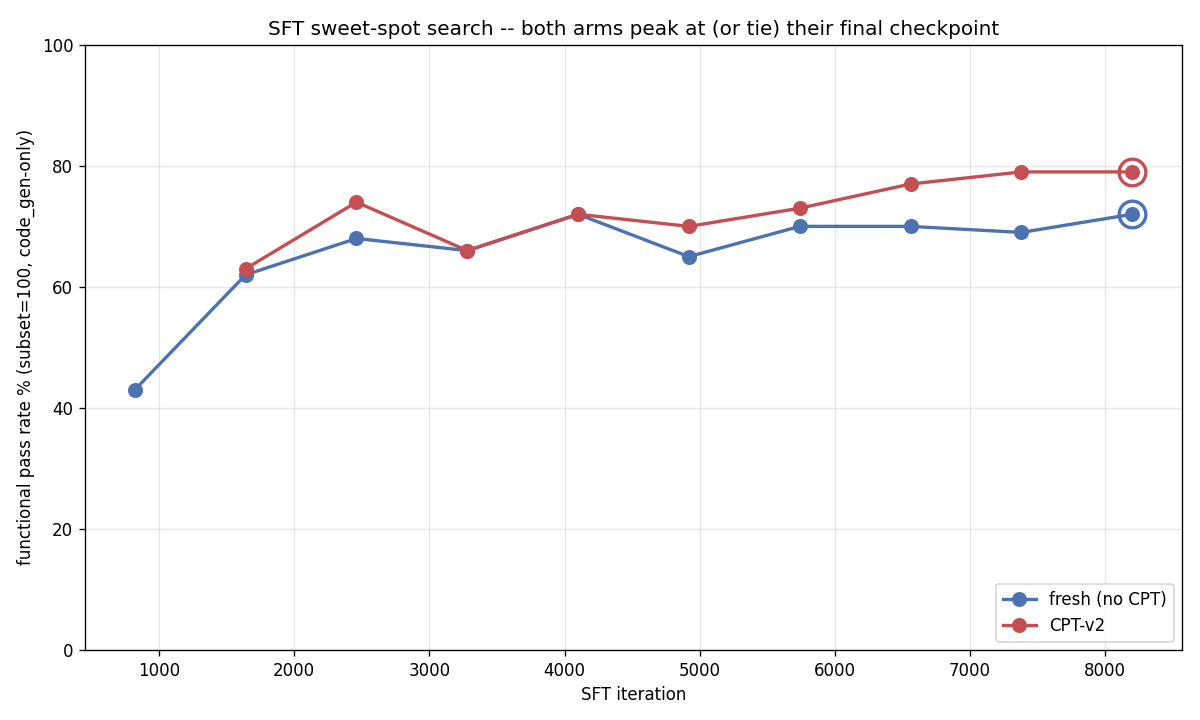
\includegraphics[width=\linewidth]{images/sft_sweetspot_curves.png}
      \end{center}
      \vspace{-0.4em}
      {\scriptsize\color{jsMute}SFT sweet-spot search: neither arm would have gained from stopping early --- the peak checkpoint ties the final one in both.}
    \end{column}
  \end{columns}
\end{frame}

% ===================================================================== 5
\begin{frame}{Two variables, five arms}{Does CPT help? And which 16 of 48 blocks should carry the LoRA?}
  \vspace{0.3em}
  \begin{center}
  \small
  \begin{tabular}{lcc}
    \toprule
     & \textbf{Trailing-16} \mut{(blocks 32--47)} & \textbf{Spectrum picks} \mut{(SNR-chosen)} \\
    \midrule
    \textbf{No CPT} (fresh base)      & Arm 1 & Arm 3 \\
    \textbf{CPT-v2} (trained on trailing-16) & Arm 2 \mut{(incumbent)} & Arm 4 \mut{(union/freeze)} \\
    \textbf{CPT on Spectrum's picks}  & \mut{---} & \warn{Arm 5 (paused)} \\
    \bottomrule
  \end{tabular}
  \end{center}
  \vspace{0.8em}
  \small
  \begin{itemize}
    \item LoRA only adapts \textbf{16 of the model's 48 decoder blocks}. \texttt{mlx\_lm}'s default takes the \emph{last} 16 --- a default nobody had ever measured.
    \item Everything else is byte-identical --- rank 16, scale 2.0, dropout 0.05, 281.8M trainable parameters. \textbf{Placement changes; capacity does not.}
  \end{itemize}
\end{frame}

% ===================================================================== 6
\begin{frame}{Question 1: does CPT help?}
  \begin{columns}[T]
    \begin{column}{0.58\textwidth}
      \begin{center}
        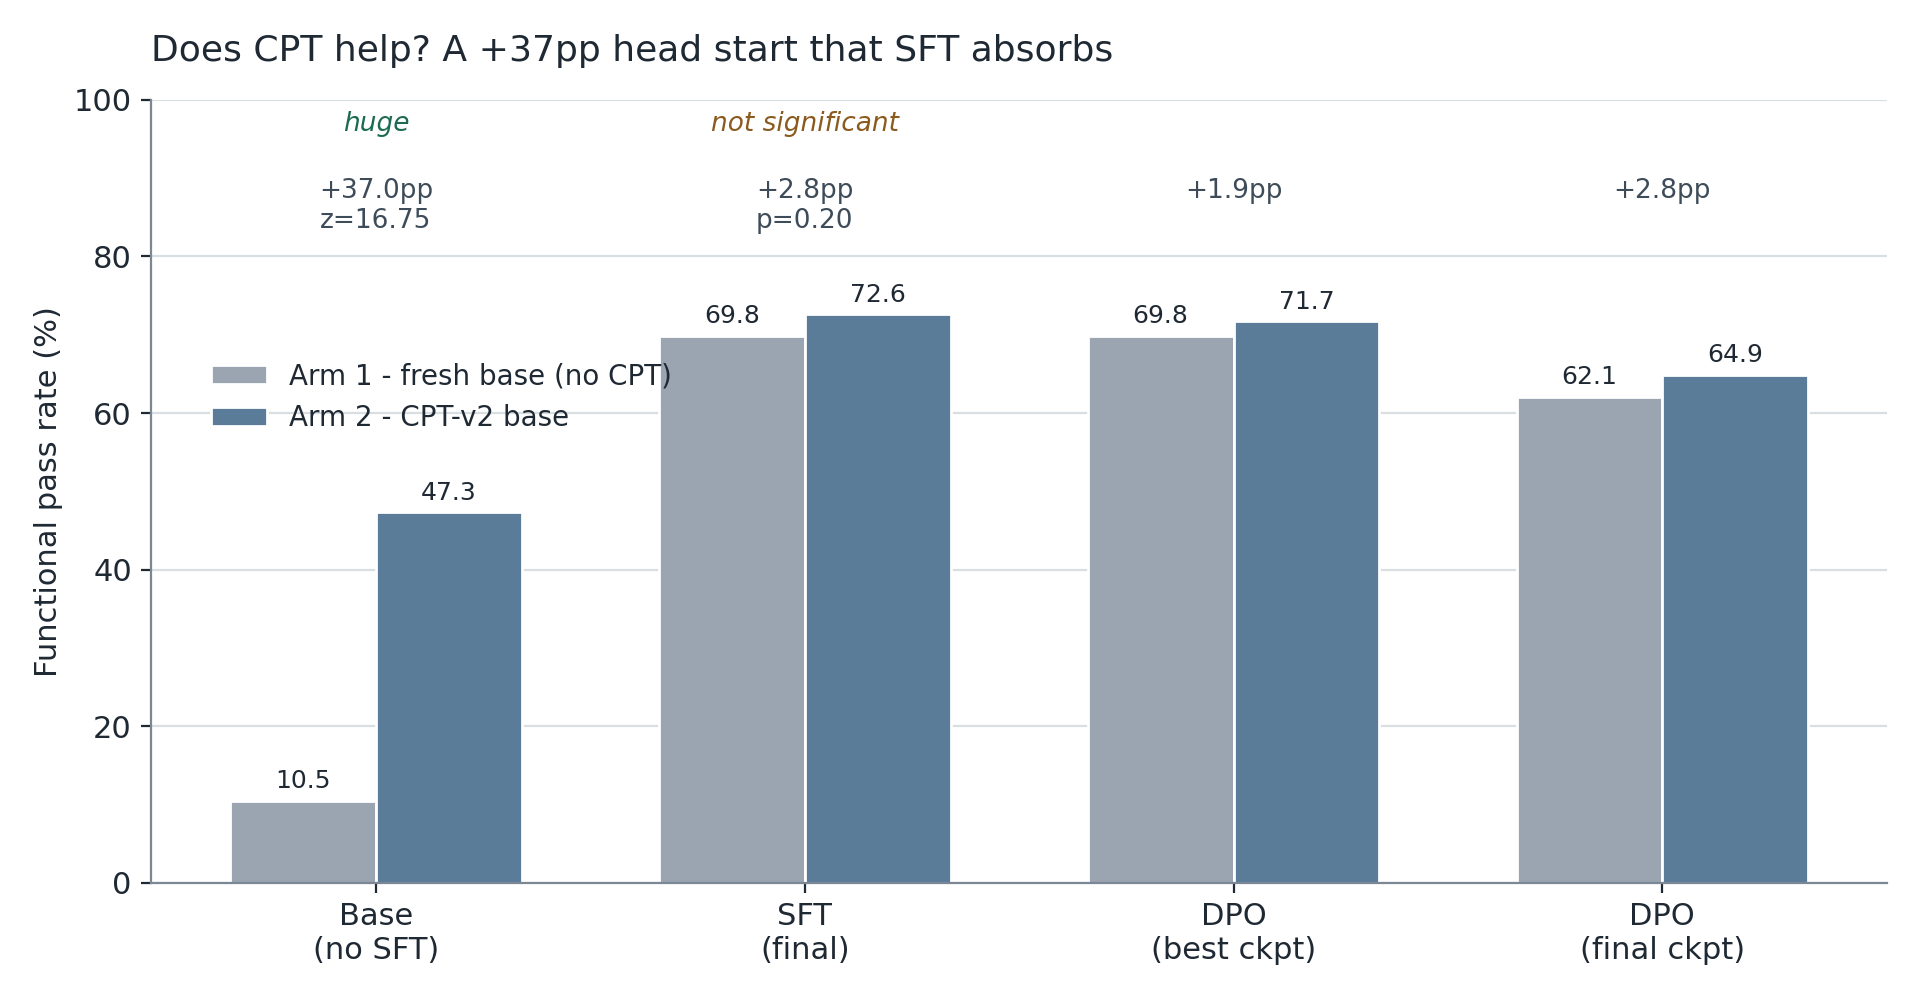
\includegraphics[width=0.98\linewidth]{images/cpt_vs_fresh_corrected.png}
      \end{center}
    \end{column}
    \begin{column}{0.40\textwidth}
      \vspace{0.4em}
      \footnotesize
      \begin{itemize}
        \item Before any task training: \good{+37.0pp} --- huge, unambiguous.
        \item After SFT: \warn{+2.8pp}, $p\approx0.20$ --- \textbf{not} significant at $n{=}855$.
        \item The three deltas are \textbf{not the same kind of fact}. +37pp is a fact; +2.8pp is a direction.
        \item CPT-v2 had already been \textbf{rejected} on its own acceptance bar --- 12 legs, all 16/16 on forgetting checks, but the semantic ceiling never moved.
      \end{itemize}
      \vspace{0.2em}
      \mut{Two-proportion $z$-test throughout --- this project's standing convention.}
    \end{column}
  \end{columns}
\end{frame}

% ===================================================================== 7
\begin{frame}{Incident 1: \texttt{mlx\_lm.fuse} was quietly deleting the training}
  \small
  \begin{columns}[T]
    \begin{column}{0.50\textwidth}
      \textbf{The symptom.} Every DPO run ``collapsed'' to $\sim$12\% --- immediate, total, identical across two arms, flat across all 13 checkpoints.
      \vspace{0.5em}\\
      \textbf{The tell.} A failure that uniform is not an optimization problem. The model was not writing \emph{bad} Jac --- it was writing React.
      \vspace{0.5em}\\
      \textbf{Root cause.} Fusing a LoRA delta into a 4-bit model dequantizes, adds, then \emph{re-quantizes} --- and re-quantization rounded the fine-grained SFT delta away. Every DPO run was training on an effectively un-SFT'd base.
    \end{column}
    \begin{column}{0.48\textwidth}
      \begin{center}
        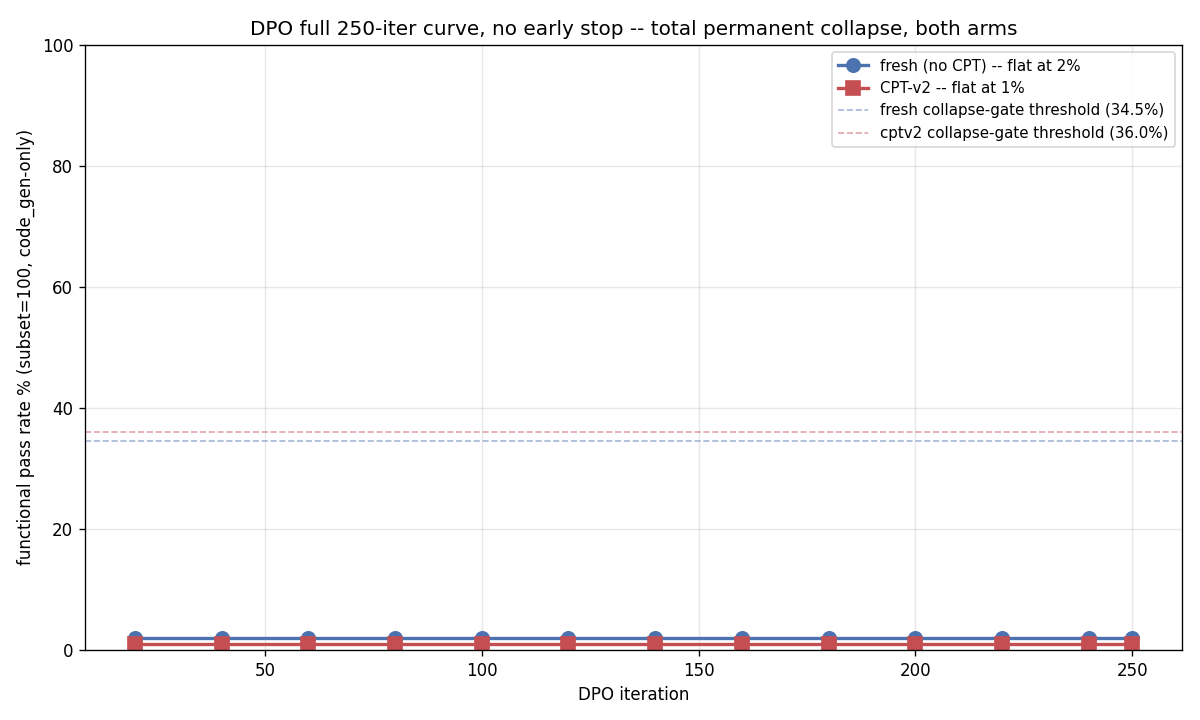
\includegraphics[width=0.90\linewidth]{images/dpo_collapse_artifact_curve.png}
      \end{center}
      \vspace{-0.7em}
      {\scriptsize\color{jsMute}The ``collapse'' --- entirely a measurement artifact.}
      \vspace{0.4em}\\
      \textbf{Fix.} Never fuse. Train DPO against the raw quantized model, seeded from the SFT adapter via \texttt{-{}-resume-adapter-file}. \good{Corrected DPO ties SFT rather than destroying it.}
    \end{column}
  \end{columns}
\end{frame}

% ===================================================================== 9
\begin{frame}{Structural vs.\ functional: CPT's fingerprint survives}
  \begin{columns}[T]
    \begin{column}{0.56\textwidth}
      \begin{center}
        
\includegraphics[width=\linewidth]{images/lora_svd_qproj_heatmap.png}
      \end{center}
    \end{column}
    \begin{column}{0.42\textwidth}
      \footnotesize
      \begin{itemize}
        \item If SFT erases CPT behaviourally, does it erase it \emph{mechanically}? A singular-value probe on the \texttt{q\_proj} LoRA updates says \textbf{no}.
        \item \textbf{CPT+SFT} tracks the standalone \textbf{CPT} adapter closely --- same rank-1 dominance, same magnitude.
        \item \textbf{Fresh SFT} sits clearly apart: more spread, roughly half the rank-1 magnitude.
        \item Layer 47 stable rank: \textbf{2.70} / \textbf{2.83} / \textbf{4.42}.
      \end{itemize}
      \vspace{0.2em}
      \good{Two differently-shaped updates reach the same pass rate.} Convergence is behavioural, not mechanistic.
    \end{column}
  \end{columns}
\end{frame}

% ==================================================================== 10
\begin{frame}{What is ``Spectrum''?}{Arcee AI's signal-to-noise layer selection, in plain terms}
  \begin{columns}[T]
    \begin{column}{0.52\textwidth}
      \begin{itemize}
        \item Take a weight matrix. Look at its singular values --- how much ``structure'' it carries in each direction.
        \item Random matrix theory (Marchenko--Pastur) tells you exactly what that spectrum would look like if the matrix were \textbf{pure noise} of the same shape and scale.
        \item Anything \emph{above} that noise floor cannot be explained by chance. It is learned structure.
        \item Rank every block by that ratio; train the top ones.
      \end{itemize}
    \end{column}
    \begin{column}{0.46\textwidth}
      \begin{block}{The intuition}
        Instead of guessing that the \emph{last} 16 blocks matter most, measure which 16 actually carry signal.
      \end{block}
      \vspace{0.5em}
      \small
      Spectrum's picks for this model:\\[0.3em]
      \texttt{[0, 22, 23, 27, 30, 34, 36, 37, 38,\\ \phantom{[}39, 41, 42, 43, 44, 45, 47]}\\[0.5em]
      Only \textbf{11 of 16} overlap the trailing slice --- and it includes \textbf{block 0}, right next to the embeddings.
    \end{column}
  \end{columns}
\end{frame}

% ==================================================================== 11
\begin{frame}{Question 2a: Spectrum on a fresh base --- a clean win}
  \begin{columns}[T]
    \begin{column}{0.55\textwidth}
      \small
      \begin{tabular}{lccc}
        \toprule
        \textbf{Stage} & \textbf{Spectrum} & \textbf{Stock} & \textbf{$p$} \\
        \midrule
        SFT       & \good{74.7\%} & 69.8\% & \good{0.023} \\
        DPO-best  & \good{74.2\%} & 69.8\% & \good{0.046} \\
        DPO-final & \good{72.7\%} & 62.1\% & \good{$<$0.0001} \\
        \bottomrule
      \end{tabular}
      \vspace{0.9em}
      \begin{itemize}
        \item Significant at \textbf{every} stage, and the margin \textbf{grows} as training proceeds.
        \item Same capacity, same recipe, same data --- only \emph{where} the adapter sits changed.
        \item The trailing-16 default was leaving real capability on the table.
      \end{itemize}
    \end{column}
    \begin{column}{0.43\textwidth}
      \begin{center}
        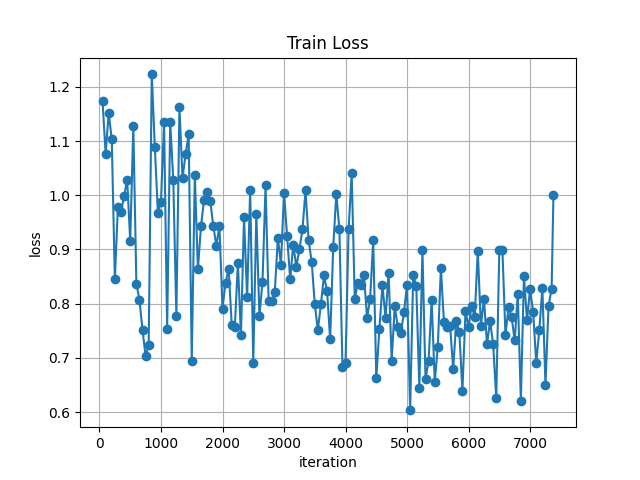
\includegraphics[width=0.92\linewidth]{images/spectrum_fresh_train_loss.png}
      \end{center}
      \vspace{-0.6em}
      {\scriptsize\color{jsMute}Arm 3 SFT training loss --- 8{,}200 iterations, no incidents on this arm.}
    \end{column}
  \end{columns}
\end{frame}

% ==================================================================== 12
\begin{frame}{Question 2b: Spectrum on top of CPT --- an honest null}
  \vspace{0.2em}
  \begin{columns}[T]
    \begin{column}{0.48\textwidth}
      \small
      \begin{tabular}{lccc}
        \toprule
        \textbf{Stage} & \textbf{Spectrum} & \textbf{Stock} & \textbf{$p$} \\
        \midrule
        SFT       & 70.5\% & 72.6\% & 0.34 \\
        DPO-best  & 71.7\% & 71.7\% & \mut{exact tie} \\
        DPO-final & 69.0\% & 64.9\% & \warn{0.072} \\
        \bottomrule
      \end{tabular}
      \vspace{0.8em}
      \begin{itemize}
        \item No stage clears $p<0.05$. One stage is even mildly negative.
        \item Reported as-is, not spun --- an asymmetric result, not a clean win.
      \end{itemize}
    \end{column}
    \begin{column}{0.50\textwidth}
      \begin{block}{Why this arm is not a fair test}
        CPT-v2 had trained blocks 32--47. Spectrum wants a \emph{different}, non-contiguous 16. Bolting one onto the other required converting the 21-block \textbf{union}, loading CPT-v2 into all of them, \textbf{freezing} the 5 CPT-only blocks, training 16, then merging the frozen 5 back into every artifact.
      \end{block}
      \vspace{0.3em}
      \small That union/freeze machinery is a \textbf{confound}, not just complexity --- and it is exactly what Arm 5 exists to remove.
    \end{column}
  \end{columns}
\end{frame}

% ==================================================================== 13
\begin{frame}{The asymmetry, in one picture}
  \begin{center}
    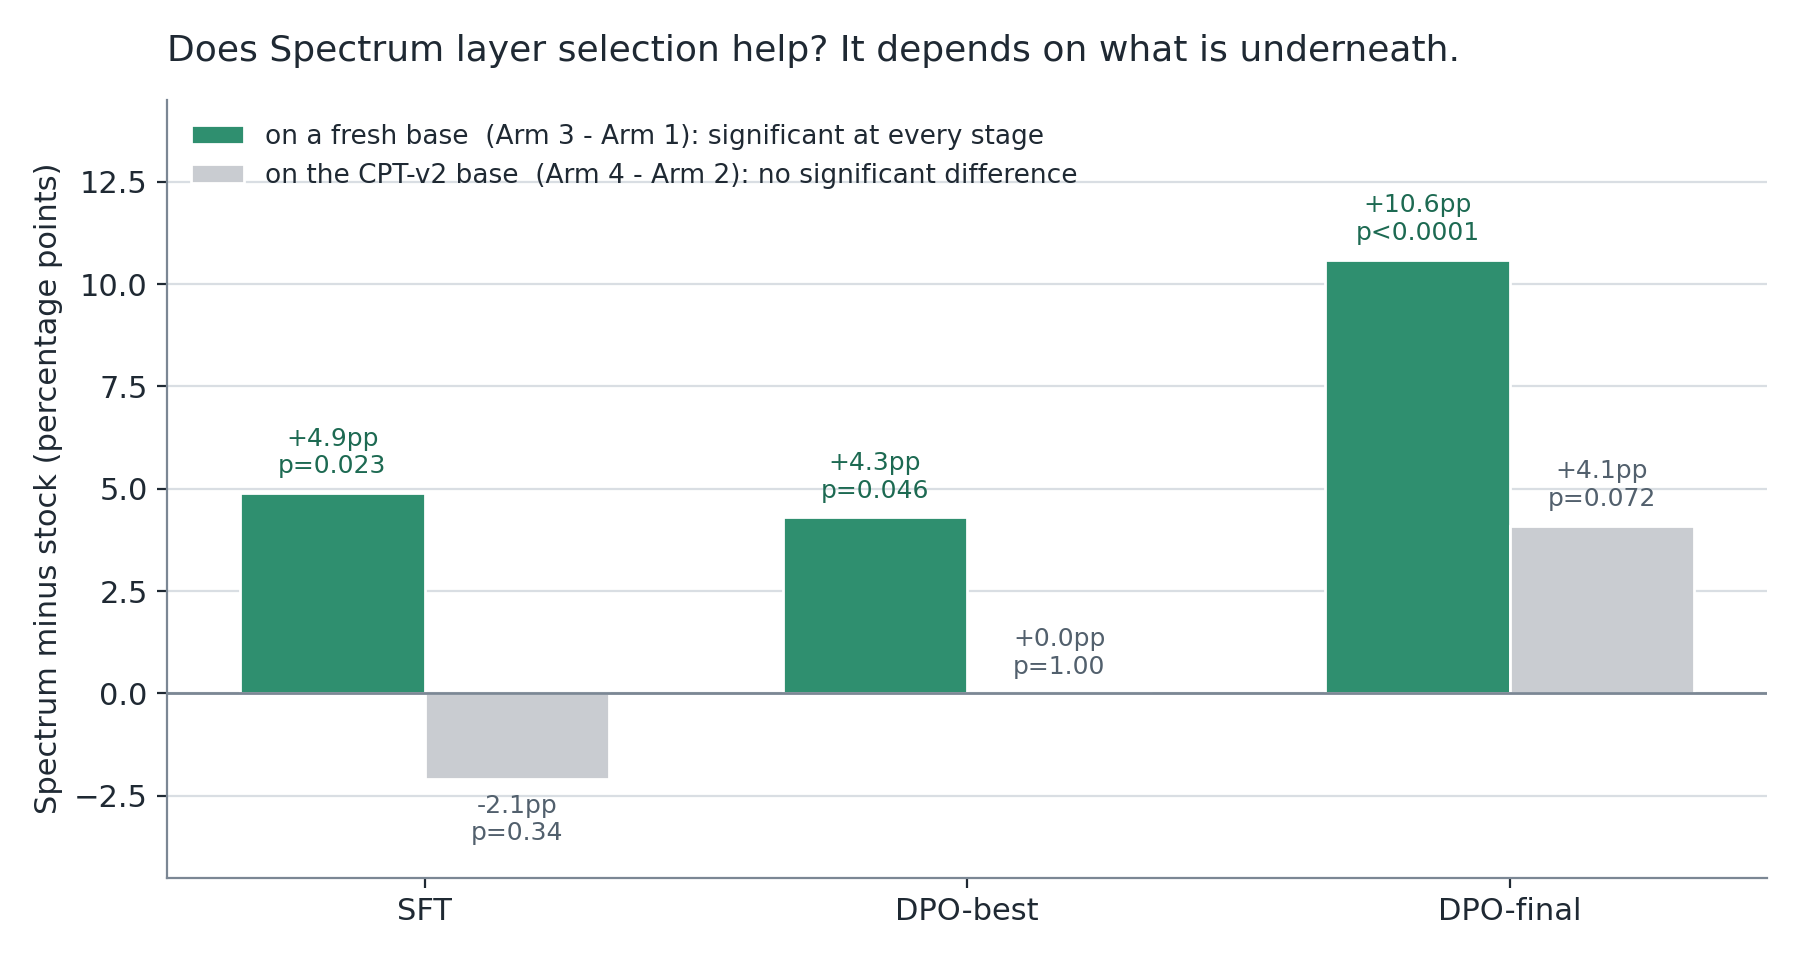
\includegraphics[width=0.72\textwidth]{images/spectrum_delta_asymmetry.png}
  \end{center}
  \vspace{-0.3em}
  \begin{center}
    \small Spectrum is a real lever \textbf{when there is no prior adaptation to work around}.\\
    On this evidence it is not a reliable lever once a CPT stage has already reshaped the same layer range.
  \end{center}
\end{frame}

% ==================================================================== 14
\begin{frame}{Incident 2: a lazy memory-map silently zeroed a trained adapter}
  \small
  \begin{columns}[T]
    \begin{column}{0.50\textwidth}
      \textbf{The symptom}
      \begin{itemize}
        \item An 8{,}200-iteration run finished clean, exit 0, normal loss curve.
        \item Every trainable LoRA weight loaded back as \textbf{exactly zero}. No error, no warning.
      \end{itemize}
      \vspace{0.5em}
      \textbf{The diagnostic that cracked it}
      \begin{itemize}
        \item The \textbf{frozen} keys were fine; only the \textbf{trained} keys were zero.
        \item Frozen keys came from a \emph{different} file. Trained keys came from the file the merge step overwrote in place.
      \end{itemize}
    \end{column}
    \begin{column}{0.48\textwidth}
      \begin{block}{Root cause}
        \texttt{mx.load()} on a safetensors file returns a \textbf{lazy memory map}. Writing back to the same path before those arrays are evaluated truncates the mmap they are still reading from.
      \end{block}
      \vspace{0.4em}
      \textbf{The fix --- one line:}
      \vspace{0.2em}\\
      {\small\texttt{trained = dict(mx.load(f))}}\\
      {\small\texttt{\good{mx.eval(list(trained.values()))}}}\\
      {\small\texttt{\# ...then write}}
      \vspace{0.6em}\\
      \small A generalizable MLX gotcha: \textbf{never read-then-overwrite a safetensors path without \texttt{mx.eval()} in between.}
    \end{column}
  \end{columns}
\end{frame}

% ==================================================================== 15
\begin{frame}{Four completed arms, side by side}
  \begin{center}
    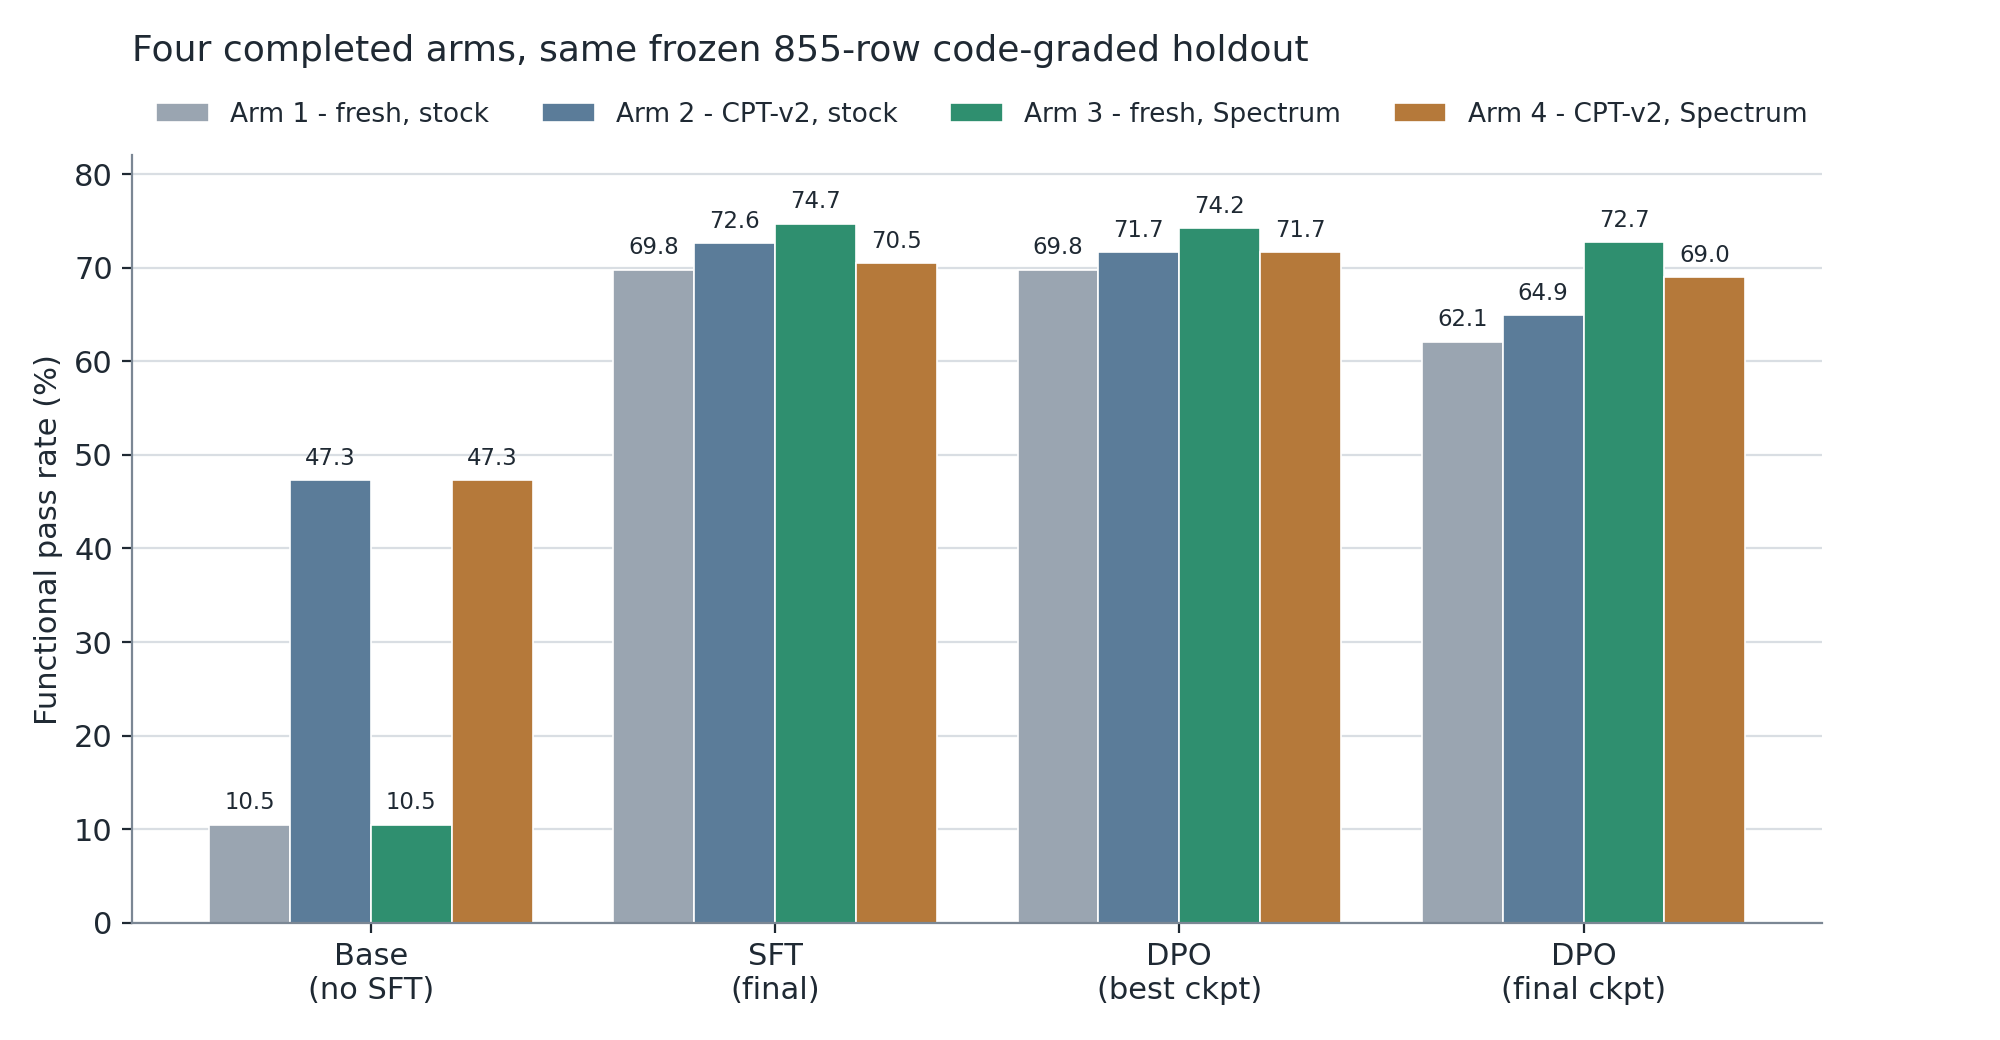
\includegraphics[width=0.82\textwidth]{images/four_arms_summary.png}
  \end{center}
  \vspace{-0.4em}
  \begin{center}
    \small Best result to date: \good{Arm 3 --- fresh base + Spectrum layer selection, 74.7\% after SFT}.\\
    \mut{All four arms scored on the identical frozen holdout, so every bar is directly comparable.}
  \end{center}
\end{frame}

% ==================================================================== 16
\begin{frame}{What is ahead: Arm 5}{The one experiment that decides how to read Arm 4}
  \small
  \begin{columns}[T]
    \begin{column}{0.50\textwidth}
      \textbf{The open question}
      \begin{itemize}
        \item Was Arm 4's null caused by the \textbf{union/freeze confound} --- CPT on one layer set, SFT/DPO on another?
        \item Or does Spectrum genuinely stop helping once \emph{any} CPT is in the chain?
      \end{itemize}
      \vspace{0.4em}
      \textbf{The design}
      \begin{itemize}
        \item Re-run CPT itself on Spectrum's exact picks: one continuous 16-block lineage, base $\rightarrow$ CPT $\rightarrow$ SFT $\rightarrow$ DPO.
        \item No union, no freeze, \textbf{no merge step anywhere} --- which removes the entire Incident-2 bug class.
      \end{itemize}
    \end{column}
    \begin{column}{0.48\textwidth}
      \textbf{Status: \warn{paused, cleanly, resumable}}
      \begin{itemize}
        \item Driver and downstream tree built; 5 pre-existing bugs found and fixed; 70 tests passing.
        \item All 3 pre-flight gates passed on the real 30B model --- peak memory \textbf{30.1\,GB}, $\sim$6\,GB under this machine's ceiling.
        \item Launched, ran leg 1, stopped intentionally before any checkpoint was written.
      \end{itemize}
      \vspace{0.3em}
      \mut{\textbf{Honest budget:} Spectrum includes block 0, so backprop traverses all 48 blocks --- a measured 1.59$\times$ slowdown. $\sim$26--30\,h for CPT alone, $\sim$37--41\,h end to end.}
    \end{column}
  \end{columns}
\end{frame}

% ==================================================================== 17
\begin{frame}{Jac Model Studio (JMS)}{The other half: a local ML workbench, written entirely in Jac}
  \begin{columns}[T]
    \begin{column}{0.44\textwidth}
      \scriptsize
      \begin{itemize}
        \item Full-stack Jac --- 34 server modules, 65 client components, $\sim$29k lines. Native desktop app; no browser, API in-process.
        \item \textbf{Two surfaces:} the \emph{Experiments} lab, and the \emph{JMS} product pipeline --- \textbf{sources $\rightarrow$ generate $\rightarrow$ curate $\rightarrow$ train $\rightarrow$ eval/chat}.
        \item \textbf{Job engine:} detached subprocesses, a heavy-GPU lock, job state on disk that survives server restarts.
        \item \textbf{Grounded AI assistant} over MLX / Claude / OpenAI, with full-app-state context and agentic actions.
        \item Graph-persistent, per-user roots, JWT auth, Spheron cloud GPUs.
      \end{itemize}
    \end{column}
    \begin{column}{0.54\textwidth}
      \begin{center}
        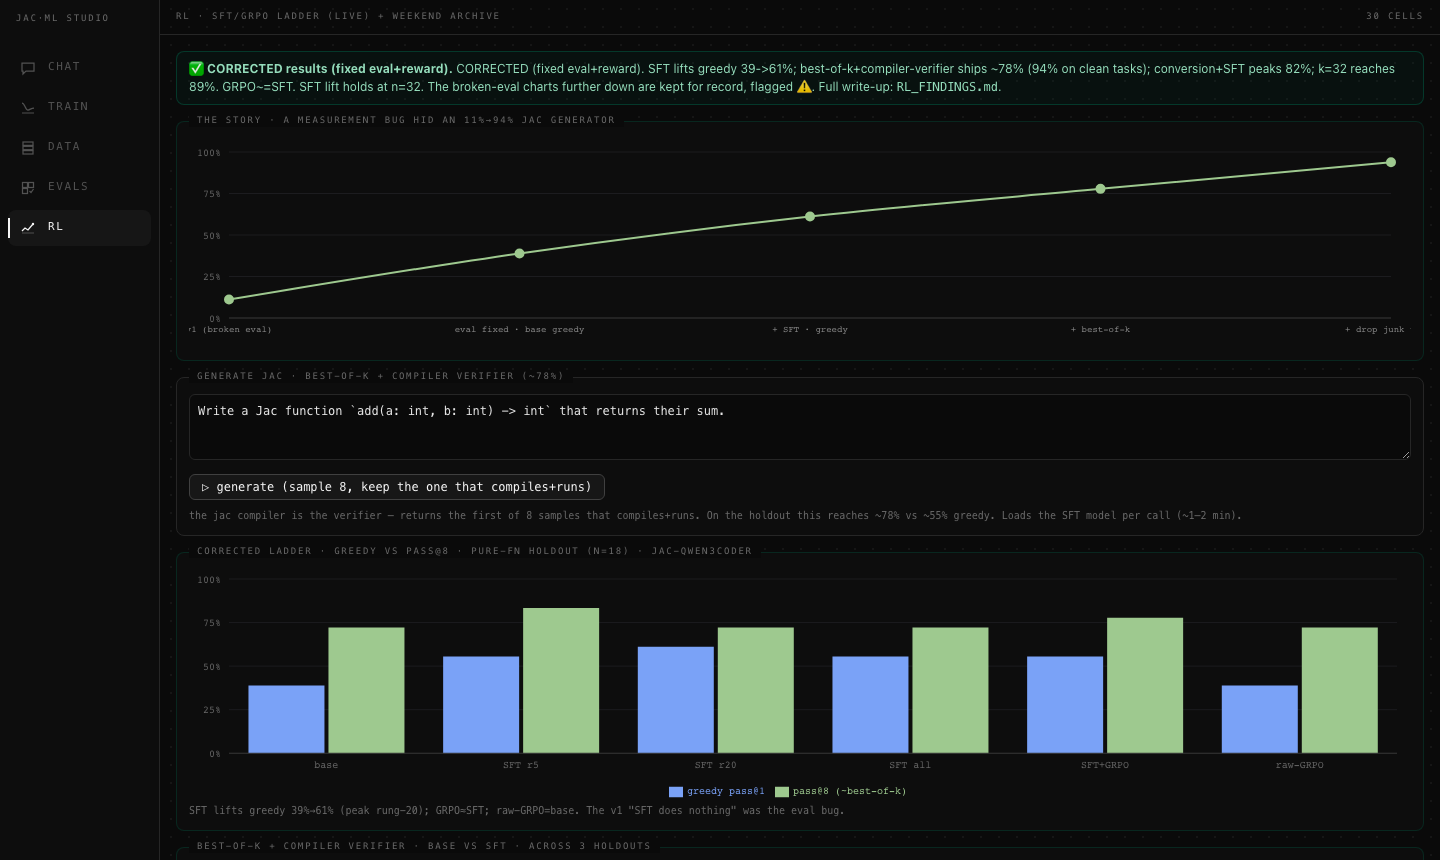
\includegraphics[width=0.96\linewidth]{images/jms_experiments_surface.png}
      \end{center}
      \vspace{-0.5em}
      {\scriptsize\color{jsMute}The Experiments surface, live --- an earlier capture from the RL/GRPO phase.}
    \end{column}
  \end{columns}
\end{frame}

% ==================================================================== 18
\begin{frame}{JMS: recent work and what is next}
  \scriptsize
  \begin{columns}[T]
    \begin{column}{0.48\textwidth}
      \textbf{Recent (July--August 2026)}
      \begin{itemize}
        \item One design system replacing 5 dormant themes and a dead 7-theme switcher: light/dark, glass overlays, one accent colour.
        \item Workspaces group projects; the Experiments side seeds one per phase (SFT/DPO, RL, CPT, CPT-SFT).
        \item Assistant matured: streaming, persistent history, markdown tables, a local Gemma 3 4B slot loading in $\sim$3\,s.
        \item Accessibility pass: command palette, shortcuts, focus traps, toasts, job watch.
      \end{itemize}
      \vspace{0.2em}
      \textbf{Next}
      \begin{itemize}
        \item Confirm-reset hook on the irreversible cloud-terminate action; remaining ARIA hints.
        \item Exercise the untested paths: a real local model load, and the Claude-dependent success paths.
      \end{itemize}
    \end{column}
    \begin{column}{0.50\textwidth}
      \textbf{The live verification sweep (August 2026)}
      \begin{itemize}
        \item $\sim$20 scripted headless-browser sessions: 48 experiment screens, both themes, 6 overlays, a 234-action endurance run.
        \item \good{Zero console errors, zero uncaught page errors, zero 4xx/5xx.}
        \item Cold start \textbf{336--347\,ms} to interactive across 8 fresh contexts.
        \item Focus traps held on 5 overlays, zero escapes.
      \end{itemize}
    \end{column}
  \end{columns}
\end{frame}

% ==================================================================== 19
\begin{frame}{Takeaways}
  \begin{itemize}
    \item \textbf{SFT is the workhorse.} It takes this model from 10.5\% to $\sim$70--75\%. Everything else is a modest edit on top of that.
    \item \textbf{CPT's gift gets absorbed.} A +37pp head start on the raw model becomes a statistically invisible +2.8pp once SFT lands --- though its \emph{structural} fingerprint is still measurable in the weights.
    \item \textbf{Unexamined defaults cost real points.} Simply moving the LoRA to SNR-chosen blocks bought \good{+4.9pp} at zero extra capacity or cost.
    \item \textbf{But the same lever failed on a different base.} Reported as a null, not buried --- and Arm 5 is designed to find out why.
    \item \textbf{Two silent-failure bugs, both in the measurement path, not the science.} A re-quantization that erased a delta, and a lazy mmap that zeroed a whole adapter. Neither raised an error. Both changed conclusions.
    \item \textbf{Design out the bug class, not the bug.} Arm 5 has no merge step at all --- so Incident 2 cannot recur there.
  \end{itemize}
\end{frame}

% ==================================================================== 20
\begin{frame}{Next steps}
  \small
  \begin{columns}[T]
    \begin{column}{0.49\textwidth}
      \textbf{Experiments}
      \begin{enumerate}
        \item Resume Arm 5's 12-leg CPT run ($\sim$26--30\,h, resumable in chunks).
        \item Run its SFT ($\sim$3.3\,h) and DPO ($\sim$1.2\,h) stages plus evals.
        \item Publish the three-way report: six $z$-tests, Arm 5 vs Arms 2 and 4 at each stage --- with the conclusions pre-committed before the numbers land.
        \item Open follow-ups: more preference data for DPO (654 pairs is thin), and whether the SVD fingerprint holds beyond \texttt{q\_proj}.
      \end{enumerate}
    \end{column}
    \begin{column}{0.49\textwidth}
      \textbf{JMS}
      \begin{enumerate}
        \item Close the remaining must-fix and should-fix items from the verification sweep.
        \item Cover the deliberately-untested paths end to end.
        \item Longer horizon: cloud dispatch and real log parsers for non-MLX backends; a dynamic section registry; per-user workspace isolation.
      \end{enumerate}
    \end{column}
  \end{columns}
\end{frame}



% =====================================================================
%  PART 2 --- NightShift: an autonomous overnight agent harness
%  Appended 2026-08-04. The first 20 slides above are untouched.
% =====================================================================

% the running footer follows the deck into its second half
\title[NightShift: an overnight agent harness]{NightShift}

% ==================================================================== 21
\begin{frame}[plain]
  \vfill
  \begin{center}
    {\color{jsPrimary}\rule{0.16\textwidth}{2pt}}\\[1.1em]
    {\large\color{jsMute}Part 2}\\[0.4em]
    {\usebeamerfont{title}\color{jsPrimary}NightShift}\\[0.6em]
    {\large\color{jsInk}An autonomous overnight agent harness ---\\and the night it taught us what a ceiling isn't}\\[1.6em]
    {\footnotesize\color{jsMute}A different project, a different failure mode.\\
     Every figure is measured from the harness's own artifacts.}
  \end{center}
  \vfill
\end{frame}

% ==================================================================== 22
\begin{frame}{What NightShift is, and why it exists}
  \small
  \begin{columns}[T]
    \begin{column}{0.47\textwidth}
      \textbf{The problem}
      \begin{itemize}
        \item \texttt{jaseci-labs/jac}: $\sim$\textbf{365{,}000 lines} of Jac, eleven packages, a compiler written in the language it compiles.
        \item It accrues the debt nobody is paid to fix: dead code, abstractions that were right two refactors ago, archetypes no test touches.
        \item Each item is small, local, mechanically verifiable, independently shippable --- and nobody wants to supervise it turn by turn.
      \end{itemize}
    \end{column}
    \begin{column}{0.51\textwidth}
      \textbf{What it does}
      \begin{itemize}
        \item Headless Claude Code sessions against the repo, \textbf{23:00--07:00}, unattended.
        \item Four rotating audit lenses $\rightarrow$ selection $\rightarrow$ one branch and one fresh agent per theme.
        \item Every branch runs a \textbf{local replica of upstream CI} --- the CI a fork PR cannot reach. Not green, deleted.
        \item Survivors open as \textbf{draft} PRs; \texttt{ns\_gh\_write} refuses \texttt{pr ready} and \texttt{pr merge}. \good{A human merges, or nobody does.}
      \end{itemize}
    \end{column}
  \end{columns}
  \srcnote{The design constraint behind everything downstream: it is unsupervised, so every stage has to be safe when it is wrong --- and \textbf{honest about not having run}.}
\end{frame}

% ==================================================================== 23
\begin{frame}{The pipeline, end to end}{\texttt{S0}--\texttt{S6} run nightly and unattended; \texttt{S7} is the human loop}
  \begin{columns}[T]
    \begin{column}{0.29\textwidth}
      \begin{center}
        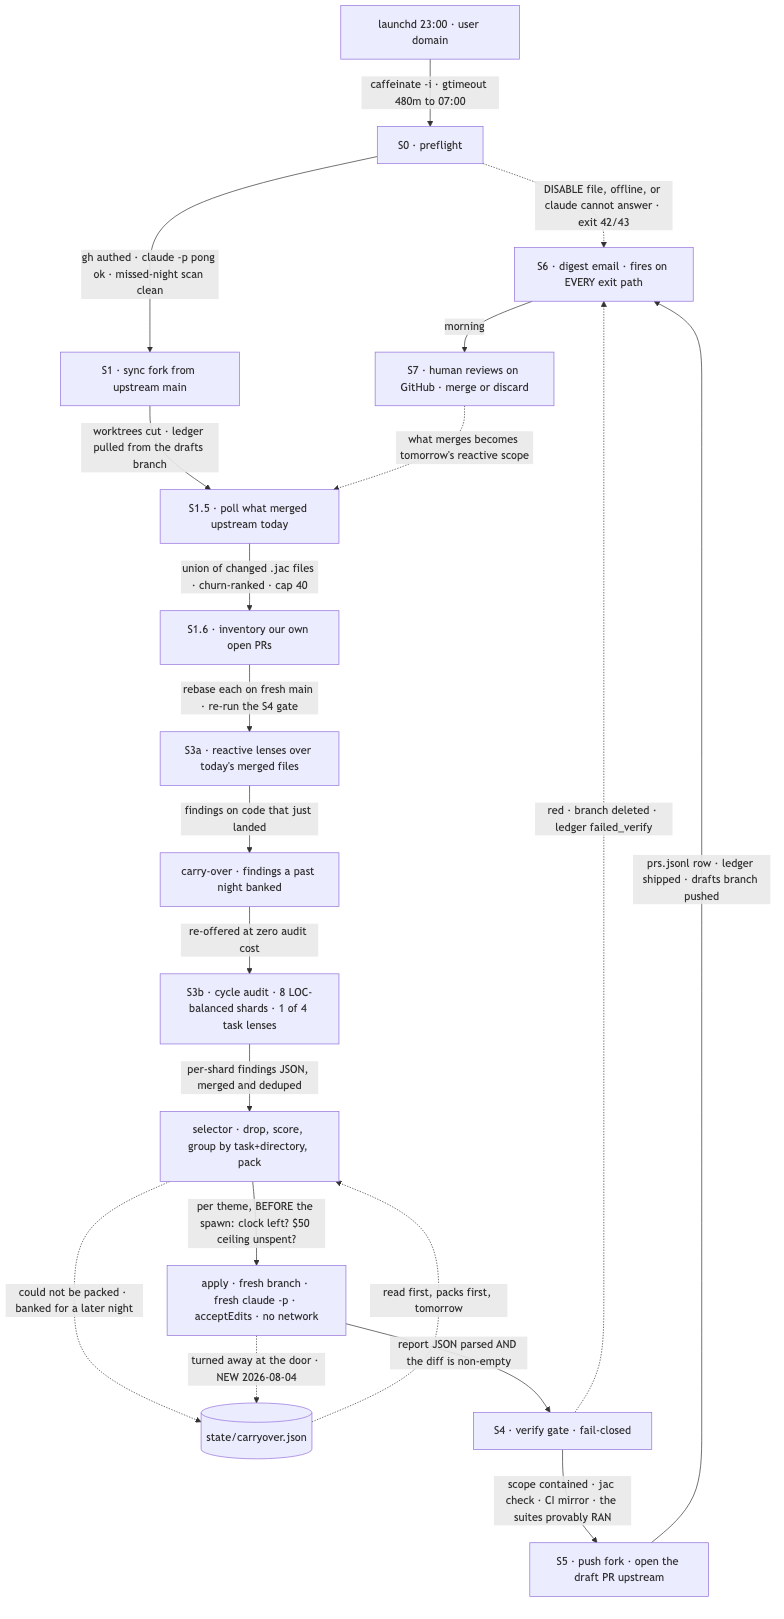
\includegraphics[height=0.68\textheight]{images/pipeline-overview.png}
      \end{center}
    \end{column}
    \begin{column}{0.67\textwidth}
      \scriptsize
      \begin{itemize}
        \item \textbf{Entry.} \texttt{launchd} at 23:00, \texttt{caffeinate}, \texttt{gtimeout 480m} in lockstep with \texttt{wallclock\_min = 480} --- the window enforced twice, by two mechanisms that cannot silently disagree.
        \item \textbf{S0 Preflight.} Lock, \texttt{DISABLE} kill file, every binary by absolute path, \texttt{gh} auth, and a literal \texttt{pong} probe proving Claude answers. Separates ``launchd fired and the run died'' from ``launchd never fired''.
        \item \textbf{S1 Sync.} Fork synced from upstream main, worktrees cut, stale branches pruned, ledger pulled down.
        \item \textbf{S1.5 Merge poll} (agent-free). Union of the \texttt{.jac} files our merged PRs touched, churn-ranked, capped at 40. If the query \emph{fails} it says so --- it does not report an empty answer.
        \item \textbf{S1.6 PR inventory} (agent-free, before any new work). Rebase our open PRs, re-run the S4 gate. \textbf{Existing PRs outrank fresh findings.}
      \end{itemize}
      \mut{There is deliberately no \texttt{S2}: the tier-1 autofix stage was retired 2026-07-30, and the gap is kept so older log lines still read true.}
    \end{column}
  \end{columns}
\end{frame}

% ==================================================================== 24
\begin{frame}{S3 $\rightarrow$ S7: audit, select, apply, gate, ship}
  \scriptsize
  \begin{columns}[T]
    \begin{column}{0.49\textwidth}
      \textbf{\color{jsPrimary}S3 --- the agentic tier}, in strict priority order
      \begin{itemize}
        \item \textbf{S3a Reactive.} Lenses over the files that merged upstream \emph{today}.
        \item \textbf{Carry-over.} Findings a past night paid to discover, re-offered at \good{zero audit cost}. \textbf{103 queued this morning.}
        \item \textbf{S3b Cycle.} Tonight's \emph{one} task --- dead-code, abstraction, maintenance, coverage --- over 8 LOC-balanced shards, read-only, \$8 cap. A session that \emph{died} is a dead lens, never salvaged into ``zero findings''.
        \item \textbf{Selection.} \texttt{selector.jac}, a pure unit-tested function: drop, score, group by \textbf{task + directory} --- not the agent's free-text hint, which once made \warn{105 groups from 112 findings}, 99 singletons.
        \item \textbf{Apply.} One theme, one branch, one fresh session: \textbf{no push, no \texttt{gh}, no network}.
      \end{itemize}
    \end{column}
    \begin{column}{0.49\textwidth}
      \textbf{\color{jsPrimary}S4 --- Verify gate}, fail-closed, cheap jobs first
      \begin{itemize}
        \item Base resolves $\rightarrow$ \textbf{scope containment} (anything outside the theme's files is treated as possible prompt injection) $\rightarrow$ \texttt{jac check} baseline-diff $\rightarrow$ CI-mirror fast jobs $\rightarrow$ the mirrored suites $\rightarrow$ \good{a positive assertion that the suites actually ran} $\rightarrow$ pre-commit $\rightarrow$ contribution rules.
        \item Anything red deletes the branch.
      \end{itemize}
      \textbf{\color{jsPrimary}S5 --- Ship}
      \begin{itemize}
        \item Push on an explicit refspec, never forced; open upstream as a \textbf{draft}, asserting on rc 0 \emph{and} a URL-shaped result --- either alone can lie.
      \end{itemize}
      \textbf{\color{jsPrimary}S6 --- Digest \quad S7 --- Human loop}
      \begin{itemize}
        \item Email built from the night's own artifacts, fired from an EXIT trap on \emph{every} exit path.
        \item Merge, discard or leave. What stays open is re-gated nightly; what merges becomes tomorrow's reactive scope.
      \end{itemize}
    \end{column}
  \end{columns}
  \srcnote{bash sequences processes, Jac owns every transformation, and there are \textbf{no Python files}.}
\end{frame}

% ==================================================================== 25
\begin{frame}{The cost model}{An unattended fleet of Opus sessions is, literally, a machine for spending money while you sleep}
  \scriptsize
  \begin{columns}[T]
    \begin{column}{0.49\textwidth}
      \textbf{Layer 1 --- per-session caps}
      \begin{itemize}
        \item \$5 per apply, \$8 per shard, \$8 per reactive lens.
        \item Separate numbers for an arithmetic reason: reactive lenses cost \textbf{\$0.139/turn} against the shards' \textbf{\$0.0638/turn} --- \textbf{2.2$\times$}. One shared cap would quietly move money from shards that produced \textbf{95 findings for \$38.36} to lenses that produced \textbf{5 for \$28.72}.
      \end{itemize}
      \vspace{0.1em}
      \textbf{Layer 2 --- the night ceiling}
      \begin{itemize}
        \item \texttt{night\_budget\_usd = 50} --- the only number that bounds spend, because \warn{a per-session cap times fifty sessions is not a brake}.
        \item The measurement behind it: one night spent \warn{\$76.55 in 97 minutes} of a 480-minute window --- \$67.36 of it audits, only \$9.19 on the eleven applies that shipped all six branches.
      \end{itemize}
    \end{column}
    \begin{column}{0.49\textwidth}
      \textbf{Layer 3 --- how spend is tracked}
      \begin{itemize}
        \item \texttt{logs/<date>/spend.txt}: one \texttt{session\_id} / \texttt{total\_cost\_usd} row per session, appended \emph{at the session}, not reconstructed afterwards.
      \end{itemize}
      \begin{block}{Both halves of that sentence are scar tissue}
        Totalling a night from the envelopes on disk gave \textbf{\$152.82 across ``50 sessions''} --- exactly double, because every \texttt{meta-} file is a byte-twin of the one it came from. Hence the \texttt{session\_id} dedupe.\\[0.3em]
        And an audit envelope is \emph{overwritten in place} by its own retry, so two real attempt-1 Opus sessions survive in no file at all.
      \end{block}
      \texttt{ns\_spend\_check} sums that ledger and \textbf{fails closed}: a missing ledger is legitimately \$0.00, but a junk one stops the work.
    \end{column}
  \end{columns}
\end{frame}

% ==================================================================== 26
\begin{frame}{The carry-over loop}{The unit of memory is the \emph{finding}: \texttt{fingerprint = sha1(file + rule)}}
  \scriptsize
  \begin{columns}[T]
    \begin{column}{0.47\textwidth}
      \textbf{Why it is load-bearing, not a nicety}
      \begin{itemize}
        \item On 2026-08-03 the night surfaced \textbf{182 findings} --- 79 fresh, \good{103 carried} --- packed \textbf{26 themes} and deferred \textbf{105 findings}.
        \item Audit money is spent \emph{at discovery}. A finding discovered and then forgotten is money burned \emph{twice}: the next audit rediscovers it and charges again.
        \item Carry-over is what converts audit spend into shipped PRs \emph{across} nights instead of within one.
      \end{itemize}
      \vspace{0.3em}
      \textbf{One governing constraint: RECONCILIATION B7}
      \begin{itemize}
        \item Carry-over belongs to the \emph{cycle} phase only. Reactive \emph{outranks} carry-over; if it also absorbed it, yesterday's deferrals would be spent twice in one night and then overwritten. \textbf{B7 forbids displacement.}
      \end{itemize}
    \end{column}
    \begin{column}{0.50\textwidth}
      \textbf{The lifecycle}
      \begin{itemize}
        \item \texttt{new} $\rightarrow$ \texttt{in\_theme} --- selected and applied. Recorded since 08-02, which stops the cycle phase re-buying what reactive already has a branch for.
        \item \texttt{new} $\rightarrow$ \texttt{deferred} --- did not fit theme, night or clock at selection, \textbf{or} (since 08-04) was turned away at apply time. Same file, same schema either way.
        \item \texttt{deferred} $\rightarrow$ \texttt{in\_theme} --- re-packed later at zero audit cost. Carried findings sort first, so the carried copy wins the \texttt{(file, rule)} dedupe and keeps its flag.
        \item \texttt{in\_theme} $\rightarrow$ \texttt{drafted} $\rightarrow$ \texttt{shipped}, or $\rightarrow$ \texttt{failed\_verify} $\rightarrow$ retry once $\rightarrow$ \texttt{rejected}.
        \item \texttt{blocked} and \texttt{file\_gone} are \textbf{terminal, and deliberately not carried}.
      \end{itemize}
    \end{column}
  \end{columns}
\end{frame}

% ==================================================================== 27
\begin{frame}{The one defect class this whole design is shaped around}
  \begin{columns}[T]
    \begin{column}{0.44\textwidth}
      \begin{center}
        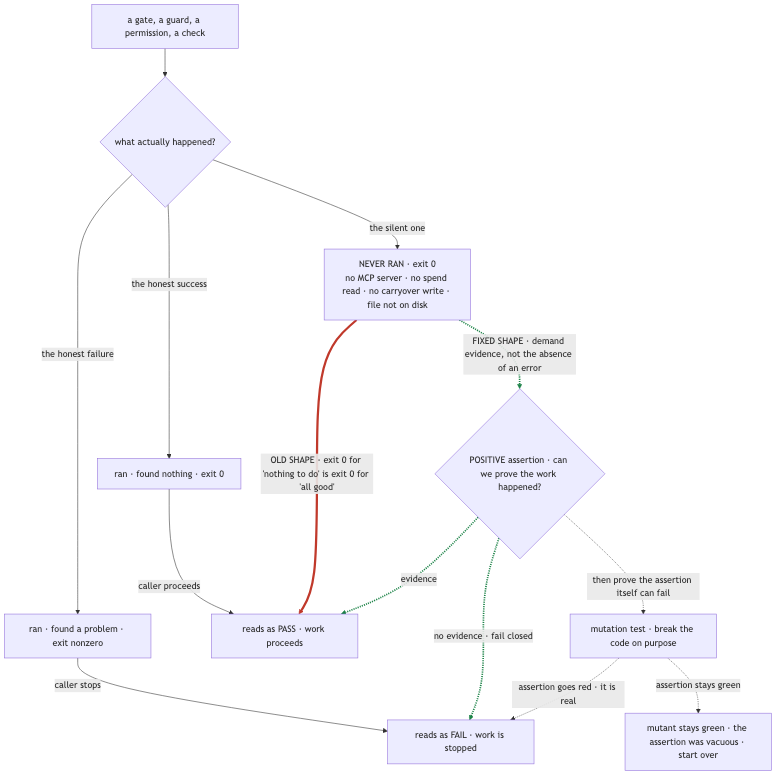
\includegraphics[width=0.96\linewidth]{images/defect-class.png}
      \end{center}
    \end{column}
    \begin{column}{0.54\textwidth}
      \vspace{0.4em}
      \begin{block}{The defect}
        \large ``Did not run'' scoring as ``passed.''
      \end{block}
      \vspace{0.6em}
      \footnotesize
      \begin{itemize}
        \item \textbf{Thirteen-plus instances} in this harness. Every one was in a gate or a guard.
        \item \warn{None was caught by a failing test} --- all were found by reading, or by an expensive night.
        \item The cause is always one shape: a command exits 0 for \emph{nothing to do} and exits 0 for \emph{all good}, and the caller cannot tell them apart.
        \item So is the countermeasure: \good{a positive assertion that the work happened}, not merely that it did not fail.
      \end{itemize}
    \end{column}
  \end{columns}
\end{frame}

% ==================================================================== 28
\begin{frame}{The catalogue --- and the sibling class}
  \scriptsize
  \begin{columns}[T]
    \begin{column}{0.52\textwidth}
      \textbf{A sample, because the range is what convinces}
      \begin{itemize}
        \item \texttt{ledger prunable} wanted five argv where the caller passed four --- so for four days every call printed usage, \warn{exited 0}, and pruned nothing.
        \item \texttt{selector}'s usage arm also exited 0, and its caller reads it on stdout. Arity drift would give an empty selection, a log line reading ``no themes tonight'', and a night reporting \emph{success} having shipped nothing. It exits \textbf{2} now.
        \item \texttt{set -e} does not fire on \texttt{for x in \$(false)}, so a malformed shard table made the audit loop iterate \warn{zero times} --- no session ever started --- and the night blamed the audit for a config error.
        \item \texttt{upsert\_theme} hard-indexed a key coverage findings do not carry: a KeyError killed the \textbf{first live night} at S3. \warn{\$17.42 spent, two finished branches thrown away.} Broken for four days, invisible because no coverage theme had ever survived an apply.
      \end{itemize}
    \end{column}
    \begin{column}{0.46\textwidth}
      \textbf{The countermeasure, everywhere}
      \begin{itemize}
        \item \texttt{assert\_suite\_ran} / \texttt{assert\_check\_ran}, with a collection floor on the test counts.
        \item S1.6 separating ``queried, zero PRs'' from ``the query failed''.
        \item S5 writing \texttt{prs.jsonl} \emph{before} its early return, so an absent file proves S5 never ran.
      \end{itemize}
      \vspace{0.3em}
      \textbf{The sibling class: assertions that cannot fail}
      \begin{itemize}
        \item \texttt{( set -e; \ldots ) || fail} is vacuous. A \texttt{grep -q} can match the comment instead of the code. A regression test can contain the bug it guards.
        \item So \good{every tripwire is paired with a mutation that must turn it red} --- which caught one tripwire looking \emph{past} the line it checked, and another whose mutant was written where \texttt{jac run} cannot load it, so ``no bad output'' was true for the wrong reason.
      \end{itemize}
    \end{column}
  \end{columns}
\end{frame}

% ==================================================================== 29
\begin{frame}{Fix 1 --- a tool grant that granted nothing}{2026-08-04, fix 1 of 4}
  \footnotesize
  \begin{columns}[T]
    \begin{column}{0.52\textwidth}
      \textbf{Problem.} Both allow-lists end with \texttt{mcp\_\_jac\_\_*} --- the Jac language server's tools, how a session gets structural answers instead of grepping for them. \textbf{That server had never been registered against the live repo path.}
      \vspace{0.5em}\\
      \textbf{Root cause.} The registration is \emph{local}, keyed by directory in \texttt{\textasciitilde/.claude.json} --- not a \texttt{.mcp.json} in the repo. A move cut a fresh clone, and a fresh clone inherits nothing. \warn{An allow-list entry naming a server that does not exist does not error; it simply matches no tool.}
      \vspace{0.5em}\\
      Every session ran without the tools it was granted, and reported success: \textbf{the grant ``did not run'', and scored as granted.}
    \end{column}
    \begin{column}{0.46\textwidth}
      \textbf{Fix.} \texttt{claude mcp add jac -{}- jac mcp} in the work tree --- now the one piece of per-machine setup a fresh deploy needs, written into \texttt{WORKFLOW.md}. \emph{The failure is silent, so the documentation is the tripwire.}
      \vspace{0.5em}
      \begin{block}{Second finding, unrelated blast radius}
        \scriptsize
        The global Claude Code settings carried a machine-wide \texttt{bypassPermissions} default. \good{NightShift's own sessions were never affected} --- it names \texttt{-{}-permission-mode} and an explicit \texttt{-{}-allowedTools} on every invocation. But it was a standing hole for \emph{every other} session on that machine. Removed.
      \end{block}
    \end{column}
  \end{columns}
\end{frame}

% ==================================================================== 30
\begin{frame}{Fix 2 --- the budget ceiling was a brake on one of two wheels}{2026-08-04, fix 2 of 4}
  \scriptsize
  \begin{columns}[T]
    \begin{column}{0.50\textwidth}
      \textbf{Problem.} \texttt{night\_budget\_usd = 50}. On 2026-08-03 the harness spent \warn{\$109.73 across 37 sessions} --- 2.2$\times$ its ceiling --- and \emph{every assertion about the ceiling stayed green.}
      \vspace{0.3em}
      \begin{center}
      \renewcommand{\arraystretch}{1.02}
      \begin{tabular}{lr}
        \toprule
        Cycle brake fired       & \$54.78 of \$50, at 00:19:30 \\
        Applies spawned after   & 16, from 00:26 to 01:56 \\
        Apply spend             & \warn{\$60.25 / 26 --- 55\%} \\
        Audit spend             & \$44.44 / 10 sessions \\
        \midrule
        Night total             & \warn{\$109.73 / 37 sessions} \\
        \bottomrule
      \end{tabular}
      \end{center}
      \vspace{0.2em}
      \textbf{Root cause.} The spend check ran only in the two audit fan-outs; the apply loop never consulted it --- a \emph{deliberate, documented and wrong} exemption. \textbf{Its premise assumed applies were 12\% of spend. They were 55\%.}
    \end{column}
    \begin{column}{0.48\textwidth}
      \begin{center}
        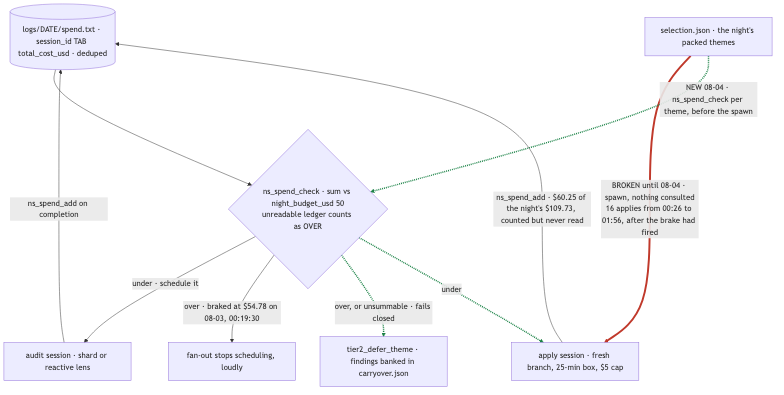
\includegraphics[width=0.80\linewidth]{images/budget-guard-before-after.png}
      \end{center}
      \vspace{-0.1em}
      \warn{A ceiling that governs one of two spending paths is not a ceiling.}
      \vspace{0.3em}\\
      \textbf{Fix.} The apply loop now runs the same check \textbf{per theme, before every spawn}, beside the clock guard, and \textbf{fails closed}.
      \vspace{0.3em}\\
      \textbf{Verified} against the \emph{real} apply loop: a defect arm (ledger at \$99 $\rightarrow$ never spawns), a fails-closed arm (junk ledger), and \good{a positive control} (at \$1 it \emph{must} spawn --- else ``no session started'' passes vacuously).
    \end{column}
  \end{columns}
\end{frame}

% ==================================================================== 31
\begin{frame}{Fix 3 --- carry-over remembered one way to fail, out of several}{2026-08-04, fix 3 of 4}
  \scriptsize
  \begin{columns}[T]
    \begin{column}{0.46\textwidth}
      \begin{center}
        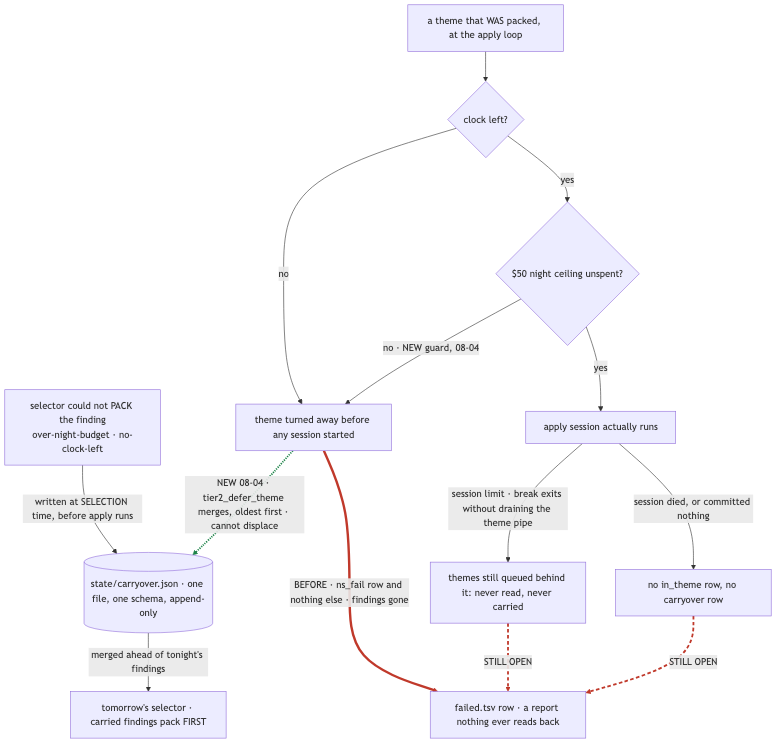
\includegraphics[width=0.97\linewidth]{images/carryover-before-after.png}
      \end{center}
    \end{column}
    \begin{column}{0.52\textwidth}
      \textbf{Problem.} \texttt{carryover.json} only ever held findings the selector \textbf{could not pack in the first place}. A theme that \emph{was} packed and was then turned away at the apply loop's door left \warn{no memory at all} --- no \texttt{in\_theme} row (written only after a session succeeds), nothing in \texttt{carryover.json} (written \emph{before} the apply loop runs), only an \texttt{ns\_fail} row that \emph{nothing ever reads back. A report, not memory.}
      \vspace{0.3em}\\
      Harmless while the only apply-time guard was the clock, which fires at the \emph{tail} of a night. \textbf{Fix 2 made it not harmless}: the cost ceiling defers themes from the \emph{front} of the loop. Shipping the brake without this fix \warn{would have turned a money leak into a silent work-deletion machine.}
      \vspace{0.3em}\\
      \textbf{Fix.} \texttt{tier2\_defer\_theme}, called from \textbf{both} apply-time guards, projects the theme's findings back into the carry-over stream. \textbf{Same file, same schema} --- a reader cannot tell an apply-time entry from a selection-time one --- and \textbf{append-only}, so it merges rather than displaces, which keeps it inside B7.
    \end{column}
  \end{columns}
\end{frame}

% ==================================================================== 32
\begin{frame}{Fix 3 --- how it is proved, and what was left open}
  \footnotesize
  \begin{columns}[T]
    \begin{column}{0.53\textwidth}
      \textbf{The strongest assertion of the day is a byte comparison}
      \begin{itemize}
        \item One finding through the \emph{real} selector twice: packed then turned away at apply, versus deferred by the selector itself. \good{The two outputs must be \texttt{cmp -s} identical.}
        \item A parallel mechanism that merely looks similar --- different keys, a missing flag, a lost fingerprint --- cannot pass that.
        \item \textbf{It appends, it does not replace:} yesterday's carry-over is seeded first and must survive. And \textbf{tomorrow can use it:} the file is fed back through the selector and must come out packed.
        \item \textbf{The false-positive arm}, the one that matters: a theme that \emph{reached} its session must \textbf{not} appear --- otherwise every finding the night shipped is re-bought tomorrow.
      \end{itemize}
    \end{column}
    \begin{column}{0.45\textwidth}
      \begin{block}{Two holes of the same shape --- known, and explicitly NOT fixed}
        \scriptsize
        \begin{enumerate}
          \item The \textbf{session-limit \texttt{break}} exits the apply loop without draining the theme pipe, so the themes behind it are never \emph{read}.
          \item A theme whose \textbf{session dies or commits nothing} still gets only an \texttt{ns\_fail} row.
        \end{enumerate}
      \end{block}
      \vspace{0.4em}
      Both are real, and both were left alone rather than bundled into a fix already touching two guards --- \good{named in the code, in \texttt{WORKFLOW.md}, and in the diagram itself.}
      \vspace{0.4em}\\
      \mut{Standing rule: a known hole gets written down where the next person will trip over it, not filed elsewhere.}
    \end{column}
  \end{columns}
\end{frame}

% ==================================================================== 33
\begin{frame}{Fix 4 --- the selector validated the paths it guessed}{2026-08-04, fix 4 of 4 --- and not the path it was given}
  \scriptsize
  \begin{columns}[T]
    \begin{column}{0.56\textwidth}
      \textbf{Problem.} A finding naming a file upstream had renamed or deleted packed a theme, took a branch and a model call, and burned a \warn{25-minute apply box to report ``no changes made.''}
      \vspace{0.4em}\\
      \textbf{Root cause.} \texttt{drop\_reason()} \emph{had} an existence check --- inside \texttt{impl\_siblings()}, which checks the candidates \textbf{it derives itself}, never the finding's own \texttt{file}. \textbf{A derived guess and a stale input are the same failure with different provenance.}
      \vspace{0.3em}\\
      And it goes stale \emph{by design}: the audit reads a clone, the clone is refreshed, upstream renames in between. On the 07-31 replay a finding still packed a theme naming \texttt{planner.jac} after upstream renamed it \texttt{query\_planner.jac}.
      \vspace{0.3em}\\
      \textbf{Fix.} It now checks the finding's own file against the tree, returning a new reason: \good{\texttt{file-gone}} --- \textbf{terminal and not carried}, since the next audit re-finds the issue at its new path, or not at all. And it \textbf{stands down when there is no tree to check}: emptying the night over a missing clone is the worse failure.
    \end{column}
    \begin{column}{0.42\textwidth}
      \begin{center}
        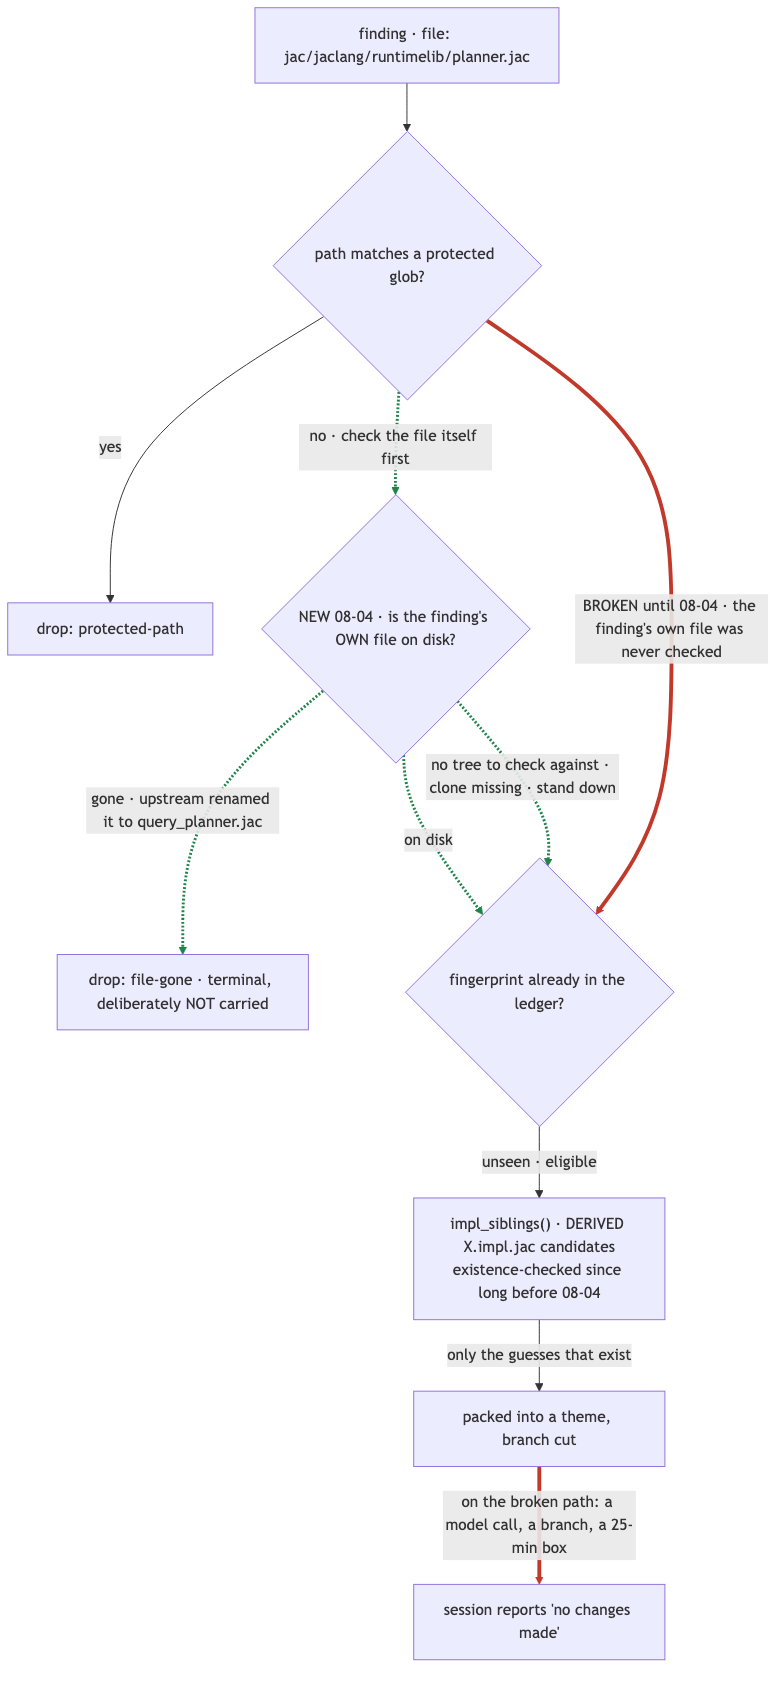
\includegraphics[height=0.34\textheight]{images/selector-file-check.png}
      \end{center}
      \vspace{-0.1em}
      \textbf{Verification.} A Jac unit test on the real 07-31 shape, three arms: the stale finding drops as exactly \texttt{file-gone}, with \textbf{no} carry-over entry; \textbf{the false-positive arm} --- the finding that \emph{is} on disk still packs, because a rule that drops everything satisfies arm 1 perfectly and costs the harness its entire output; and \textbf{the stand-down arm}, proving a missing clone cannot silently empty the night.
    \end{column}
  \end{columns}
\end{frame}

% ==================================================================== 34
\begin{frame}{What is still open}
  \footnotesize
  \begin{columns}[T]
    \begin{column}{0.50\textwidth}
      \textbf{The budget sizing decision --- deferred, not forgotten}
      \begin{itemize}
        \item \texttt{night\_budget\_usd} is still \textbf{50}. Fix 2 makes the number \emph{mean} something; it does not claim it is right.
        \item \textbf{Raise the cap} --- 08-03 produced real work at \$109.73; if that is worth it, the ceiling should say so.
        \item \textbf{Cut audit spend} --- \$44.44 bought 79 fresh findings against a queue already holding 103. \good{The bottleneck is not discovery.}
        \item \textbf{Accept audit-only nights} --- banking everything for tomorrow. A \emph{decision}, not a discovery.
        \item The data exists: cost, model, phase and findings are logged per session, so ``findings per dollar'' is a query.
      \end{itemize}
    \end{column}
    \begin{column}{0.48\textwidth}
      \textbf{The two remaining carry-over holes} --- the session-limit \texttt{break}, and the theme whose session dies or commits nothing.
      \vspace{0.5em}\\
      \textbf{A reporting gap that follows from fix 3.} \texttt{themes\_deferred} counts \emph{selection-time} deferrals only, so on a night whose apply loop hits the ceiling it \warn{undercounts the real backlog}.
      \vspace{0.5em}\\
      \textbf{Readiness, honestly.} The system is armed and unattended, and \emph{young}: the v2 cutover was 08-02, and the first live night after it died at S3 on a \texttt{KeyError}. \warn{Two of the last four nights found a defect in the harness rather than in the target repo} --- a ratio expected to fall, and \textbf{measured}, not asserted.
    \end{column}
  \end{columns}
\end{frame}

% ==================================================================== 35
\begin{frame}{Where the system stands tonight}
  \footnotesize
  \begin{itemize}
    \item \good{\texttt{bin/test-harness.sh}: 41 of 41 sections green} --- up from red at section 32 this morning.
    \item \textbf{Every fix landed today was mutation-tested} --- each new assertion was verified to go \emph{red} against the broken behaviour, not merely green against the fix. That is why they are believable at all.
    \item \textbf{The night ceiling is now a ceiling.} Both spending paths consult the same check against the same ledger, and both fail closed.
    \item \textbf{The carry-over queue holds 103 findings}, all already paid for, now fed by both deferral paths through one file, one schema, one reader.
    \item \textbf{The \texttt{jac} MCP server is registered and connected}, so the tool grants resolve to real tools; the machine-wide \texttt{bypassPermissions} default is gone.
    \item \textbf{Nights are armed}: loaded in launchd, no \texttt{DISABLE} file, window 23:00--07:00 with a 480-minute ceiling.
  \end{itemize}
  \begin{block}{The through-line, one sentence}
    \scriptsize
    Every defect closed today was the same defect --- something that did not run, and read as something that passed. The only reliable defence found here is to \textbf{demand positive evidence that work happened, then break the code on purpose.}
  \end{block}
\end{frame}


% ==================================================================== 36 (moved from end of Part 1)
\begin{frame}[plain]
  \vfill
  \begin{center}
    {\color{jsPrimary}\rule{0.16\textwidth}{2pt}}\\[1.2em]
    {\LARGE\bfseries\color{jsPrimary}Thank you}\\[0.8em]
    {\large\color{jsInk}Questions?}\\[2.0em]
    {\footnotesize\color{jsMute}Ayush \textperiodcentered\ Jaseci Labs \textperiodcentered\ August 2026}
  \end{center}
  \vfill
\end{frame}

\end{document}
